\documentclass[12pt]{article}
\usepackage{amssymb, amsmath, amsfonts, bm, graphicx, geometry}
\usepackage{tabularx, booktabs, float, enumitem, multicol, mathtools}
\usepackage{parskip} % Auto-manages paragraph spacing and removes indentations
\usepackage{siunitx}  % Eases typesetting of numbers and units
\usepackage{soul}

\geometry{margin=1in}

\begin{document}

\begin{center}
{\LARGE ESC-340 Fluid Mechanics \& Flow Systems Notes\par}
\end{center}
\hrule
\vspace{1.5em}

\section*{\fbox{2.8 Hydrostatic force on a plane surface}}
For fluid at rest, fluid pressure acts perpendicular to any surface because there is no shear stress present in a static fluid.\\\\
For example, the pressure and force distribution on an open tank is shown below:
\begin{center}
    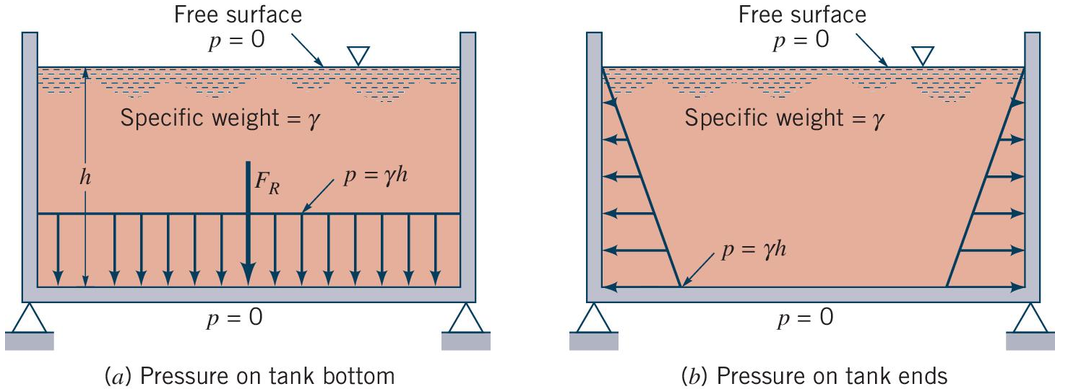
\includegraphics[width=0.7\textwidth]{2.8 Tank.png}
\end{center}
Note that if atmospheric pressure acts on both sides and bottom of the tank, it will cancel out and can be ignored (which is why we often use gage pressure). The resultant force on the bottom of tank is given by:
\[F_R = pA, \quad \text{where } p = \gamma h\]
Since the pressure is constant and uniformly distributed over the bottom, the resultant force acts through the \hl{centroid of the area}. However, for the sides of the tank the pressure varies with depth, so it's harder to determine the resultant force and its line of action.
\newpage
\subsection*{Resultant Force on a Plane Surface}
Consider the following submerged inclined plane surface below. The free surface is open to the atmosphere. We define a $xy$ coordinate system so that the surface lies on the $xy$ plane, with the origin where the plane in which the surface lies intersect the free surface.
\begin{center}
    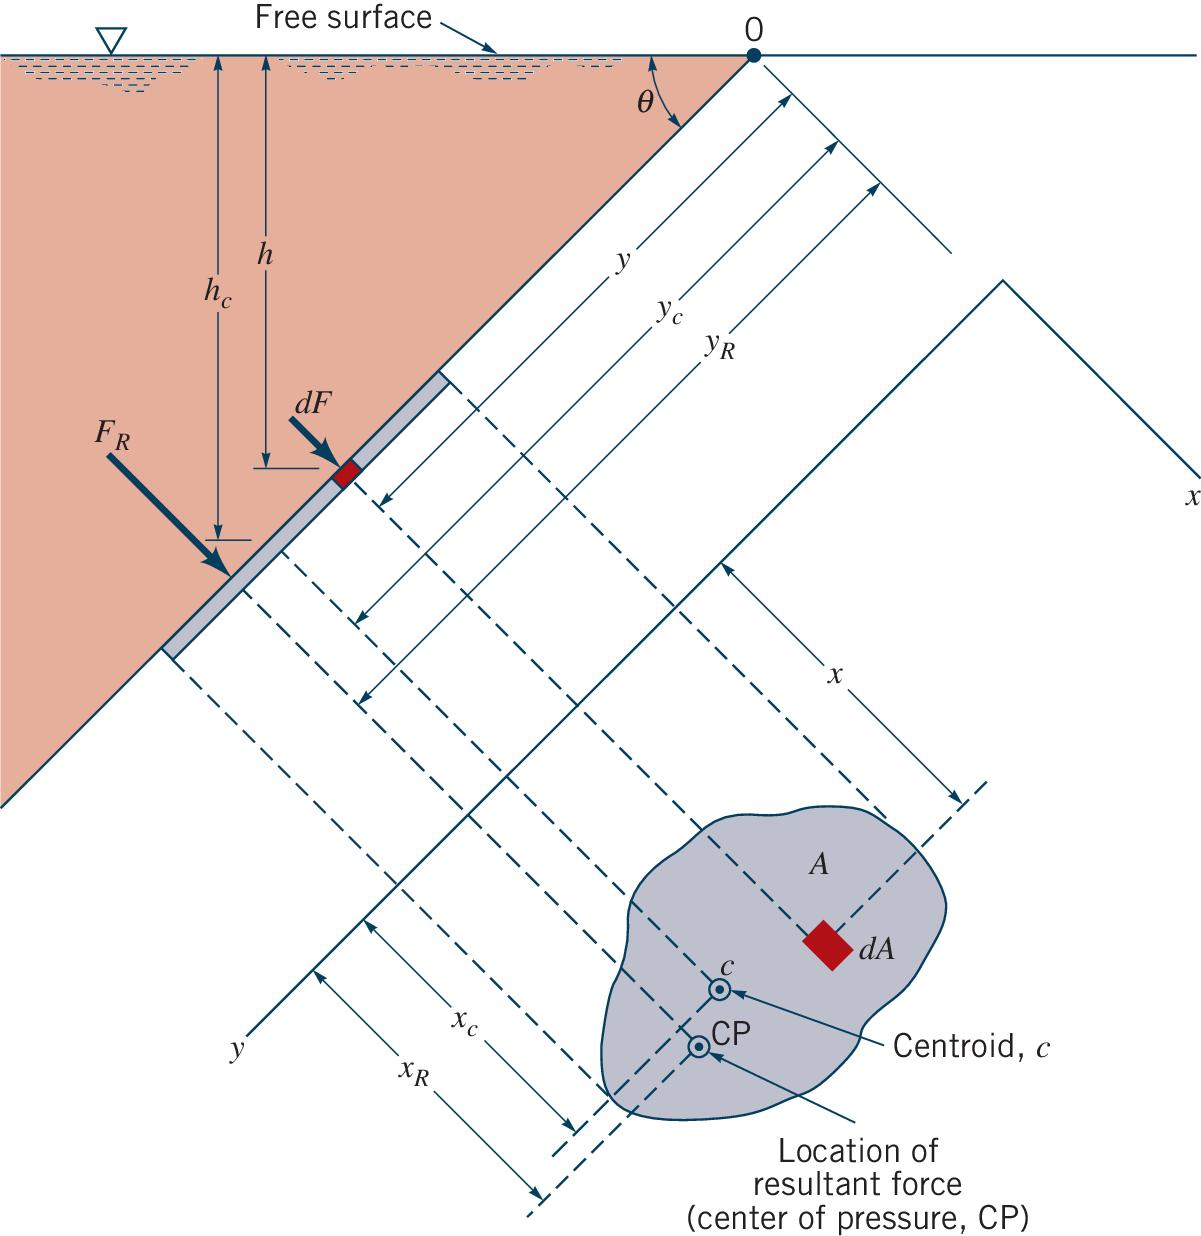
\includegraphics[width=0.7\textwidth]{2.8 Resultant Force.jpg}
\end{center}
The force due to the fluid pressure in contact with the surface is given by integrating the pressure over the area of the surface:
\[F_R = \int_A p \, dA = \int_A \gamma h \, dA\]
Where $h$ is the depth of the surface element $dA$ below the free surface ($h$ is in the vertical direction, NOT in the $y$ direction). Note that the depth $h$ can be expressed in terms of the $y$ coordinate by the angle of inclination $\theta$:
\[h = y \sin \theta\]
Also note that the integral for $F_R$ can be expressed in terms of the first moment of area of the surface about the $x$-axis:
\[Q = \int_A y \, dA= A\bar{y}\quad \text{(First Moment of Area)}\]
Where $y$ is the distance from the $x$-axis to the area element $dA$, and $\bar{y}$ is the distance from the $x$-axis to the centroid of the area. Thus, using some new notation, we can express the resultant force as:
\[F_R  = \int_A \gamma h\, dA = \int_A \gamma y \sin \theta \, dA\]
For a constant $\gamma$ and $\theta$, and $h = y \sin \theta$:
\[F_R = \gamma \sin \theta \int_A y \, dA = \gamma \sin \theta Ay_c\]
Where $\bar{y}=y_c$ is the distance from the $x$-axis to the centroid of the area along the $y$-axis. Finally:
\[\boxed{F_R = \gamma h_c A}\]
\subsection*{$y$ Coordinate of the Resultant Force}
Recall that the resultant force acts through the centroid of the area when the pressure is constant (like the bottom of the tank). However, when the plane surface is inclined, the pressure increases with depth, and the resultant force acts slightly below the centroid of the area.\\\\
We can determine the $y$ coordinate of the resultant force ($y_R$) by summing moments about the $x$-axis. The moment of the resultant force at $y_R$ is equal to the moment of the distributed pressure about the $x$-axis:
\[F_R y_R = \int_A y\, dF,\quad dF = \gamma h \, dA = \gamma y \sin \theta \, dA\]
\[\implies F_R y_R = \int_A \gamma \sin\theta y^2\,dA\]
From before, $F_R  = \gamma h_c A = \gamma \sin \theta Ay_c$. So for a constant $\gamma$ and $\theta$:
\[\gamma \sin \theta Ay_c y_R = \gamma \sin\theta \int_A y^2\,dA\]
\[\implies y_R = \frac{\displaystyle\int_A y^2\,dA}{y_c A}\]
Note that the integral in the numerator is the second moment of area about the $x$-axis, which is also known as the \textit{area moment of inertia}:
\[I_x = \int_A y^2\,dA\]
Thus, we can express the $y$ coordinate of the resultant force as:
\[y_R = \frac{I_x}{y_c A}\]
Using the parallel axis theorem, we can express $I_x$ in terms of an axis parallel to the $x$-axis that passes through the centroid of the area:
\[I_x = I_{xc} + A y_c^2\]
Thus,
\[\boxed{y_R = \frac{I_{xc}}{y_c A}+y_c}\]
Following the intuition from the beginning, since $I_{xc}/(y_c A)$ is always positive, the resultant force will always act below the centroid of the area.
\begin{center}
    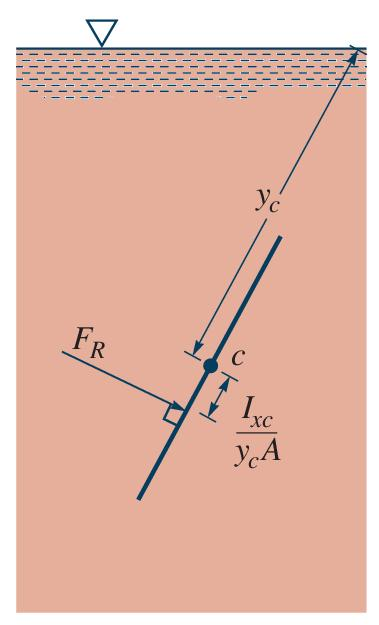
\includegraphics[width=0.4\textwidth]{2.8 y coord of resultant.jpg}
\end{center}
\underline{Note:} $y_c$ is measured from the line of intersection of the $xy$ plane with the surface, defining the angle $\theta$. However, when the $xy$ plane is horizontal and parallel to the free surface, $\theta \to 0^\circ$, and $y_c = h_c/\sin\theta \to \infty$. In this case, the term $I_{xc}/(y_c A) \to 0$, and the resultant force acts through the centroid of the area, as expected.
\newpage
\subsection*{$x$ Coordinate of the Resultant Force}
Similarly, we can determine the $x$ coordinate of the resultant force ($x_R$) by summing moments about the $y$-axis. The moment of the resultant force at $x_R$ is equal to the moment of the distributed pressure about the $y$-axis:
\[F_R x_R = \int _A x\,dF, \quad dF = \gamma h \, dA = \gamma y \sin \theta \, dA\]
\[\implies F_R x_R = \int_A \gamma \sin \theta xy\,dA\]
Since $F_R = \gamma h_c A = \gamma \sin \theta Ay_c$, for a constant $\gamma$ and $\theta$, we can divide through by $F_R$ to get:
\[x_R = \frac{\gamma \sin \theta \int_A xy\,dA}{\gamma \sin \theta Ay_c} = \frac{I_{xy}}{y_c A}\]
Like before, $I_{xy}$ is the product of inertia about the $x$ and $y$ axes. Using the parallel axis theorem, we get the general expression for the $x$ coordinate of the resultant force:
\[\boxed{x_R = \frac{I_{xyc}}{y_c A}+x_c}\]
Where $I_{xyc}$ is the product of inertia about the $x$ and $y$ axes that pass through the centroid of the area, and $x_c$ is the $x$ coordinate of the centroid of the area.\\\\
Note that if the plane surface is symmetrical about an axis parallel to either the $x$ or $y$ axis and passing through the centroid of the area, then $I_{xyc} = 0$, and $x_R = x_c$.\\\\
Together, $x_R$ and $y_R$ define the \textit{center of pressure}, which is the point where the resultant force acts on the plane surface.\\\\
\underline{Note:} For both $x_R$ and $y_R$, the center of pressure will move closer to the centroid of the area as the plane surface becomes more horizontal ($\theta \downarrow$), and thus increases $y_c$ in the denominator of both expressions. In the limit as $\theta \to 0^\circ$, $y_c \to \infty$, and the center of pressure coincides with the centroid of the area, as expected.
\newpage
\subsection*{Common Area Moments of Inertia}
\begin{center}
    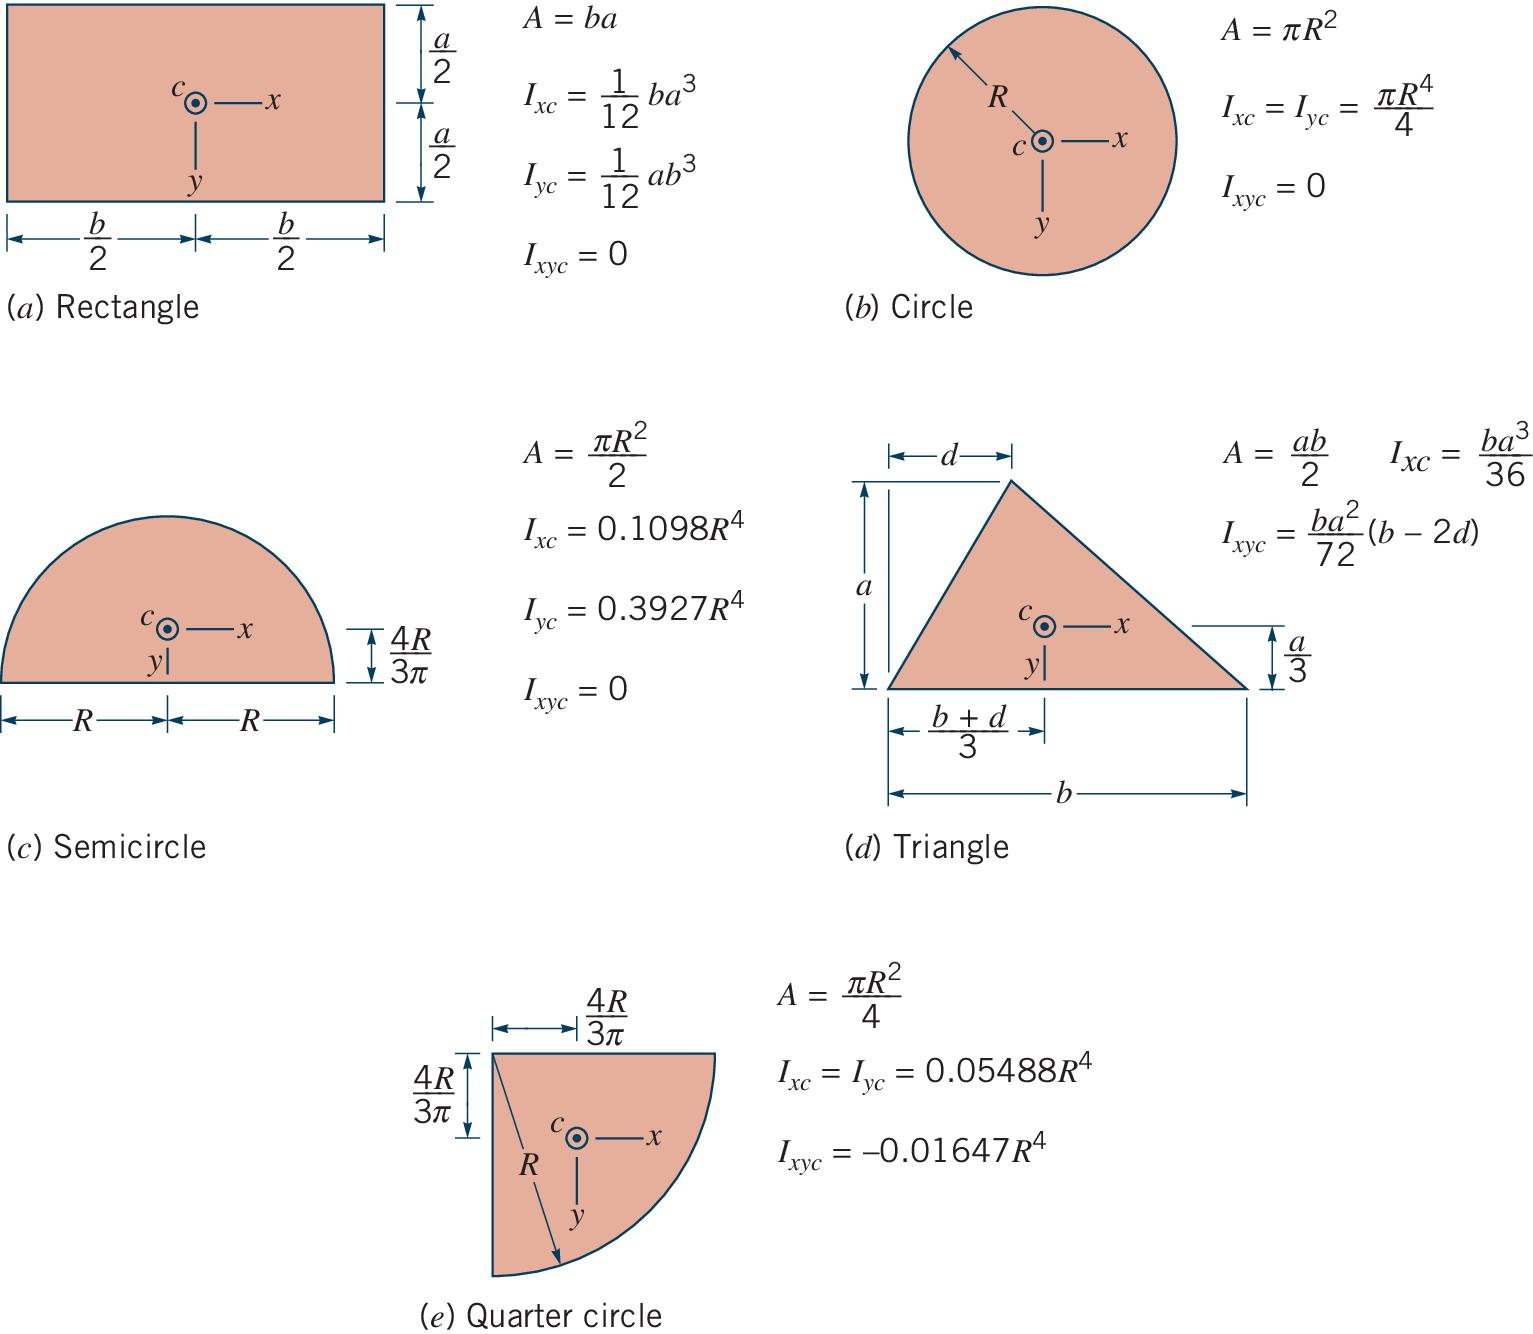
\includegraphics[width=\textwidth]{2.8 Moments of Area.jpg}
\end{center}
\newpage
\section*{\fbox{2.9 Pressure Prism}}
This section doesn't introduce any new concepts, but rather provides a graphical approach to solving for the resultant force and center of pressure on a plane surface. \hl{This approach is often convenient for rectangular surfaces, where the centroid and volume of the pressure prism can be easily determined.}\\\\
Consider the following pressure prism on a vertical plane surface with constant width $b$:
\begin{center}
    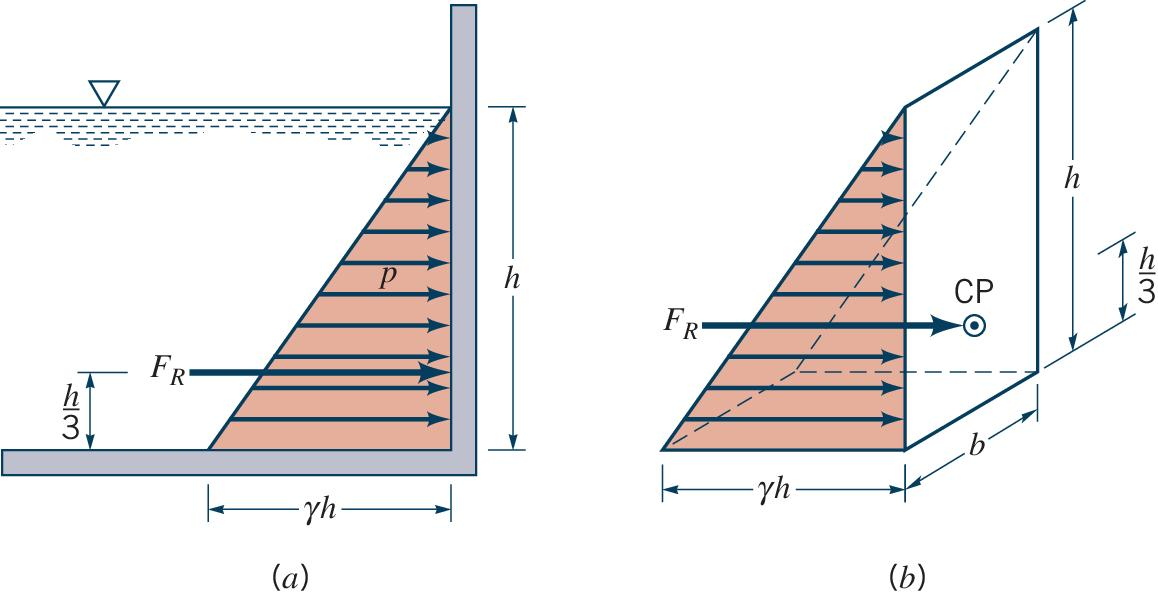
\includegraphics[width=0.7\textwidth]{2.9 Pressure Prism.jpg}
\end{center}
Since the pressure varies linearly with depth, it is zero at the free surface ($p_{min} = 0$) and maximum at the bottom of the surface ($p_{max} = \gamma h$). Thus, the average pressure on the surface is $p_{avg} = \frac{p_{min}+p_{max}}{2} = \frac{\gamma h}{2}$. The resultant force on the surface is given by:
\[F_R = p_{avg} A = \gamma \left(\frac{h}{2}\right)A\]
This is the same result as the equation $F_R = \gamma h_c A$ in section 2.8.\\\\
By forming a \textit{pressure prism} (shown in figure (b)), the resultant force can be determined graphically as the \hl{volume of the pressure prism}:
\[F_R = \text{volume} = \frac{1}{2}(\gamma h)(bh)\]
This is the same result as before as well.\\\\
The center of pressure can also be determined graphically as the \hl{centroid of the pressure prism}. The centroid of a triangle is located at a distance of $\frac{1}{3}$ from the base, so the center of pressure is located at a distance of $\frac{h}{3}$ from the bottom of the surface. This is the same result as the equation $y_R = I_{xc}/(y_c A)+y_c$ in section 2.8.\\\\
\underline{Note:} The pressure prism is always drawn starting from the free surface.
\newpage
\subsection*{Rectangular Surfaces that do not intersect the free surface}
Consider the following plane surface that does not intersect the free surface:
\begin{center}
    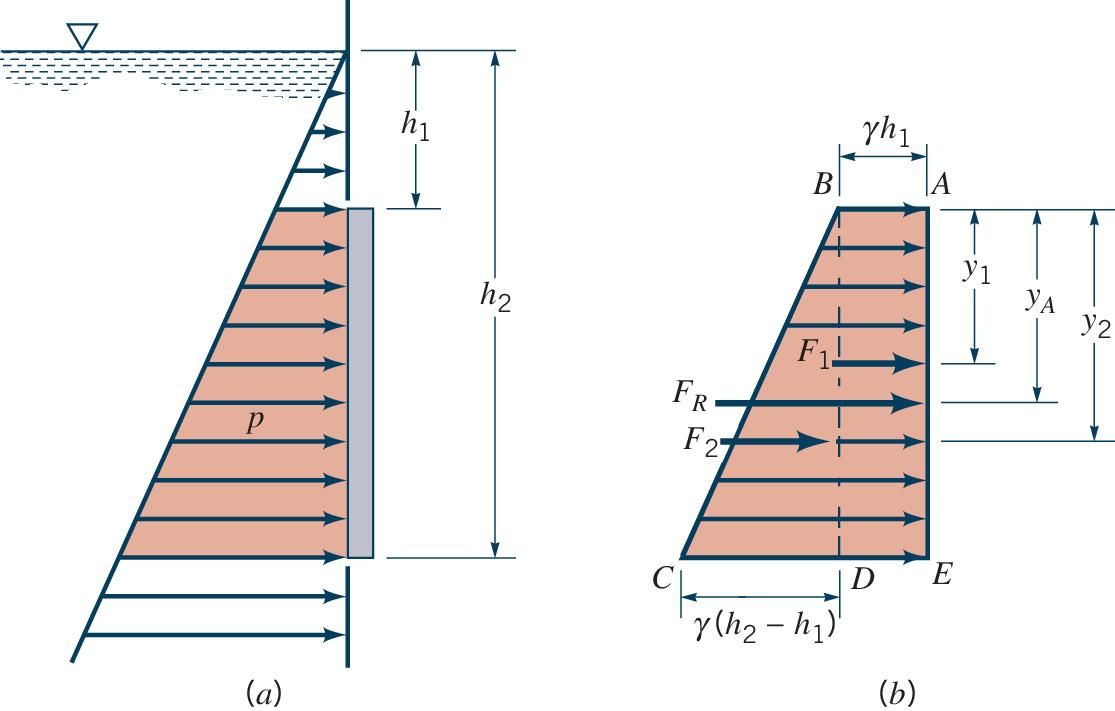
\includegraphics[width=0.7\textwidth]{2.9 No Intersection.jpg}
\end{center}
The pressure prism approach can still be used but in this case, it is trapezoidal instead of triangular. The resultant force can be found by decomposing the trapezoid into a rectangle and triangle, $ABDE$ and $BCD$, respectively. 
\[F_R = F_1 + F_2\]
The locations of the forces $F_1$ and $F_2$ can be found by taking the centroid of each shape, getting $y_1$ and $y_2$, respectively. The location of the resultant force can then be found by summing moments about a convenient axis (in this case, the axis passing through $A$):
\[F_R y_R = F_1 y_1 + F_2 y_2\]
\newpage
\subsection*{Inclined Rectangular Surfaces}
A similar approach using trapezoidal pressure prisms can be used for inclined rectangular surfaces. However, note that while it is convenient to measure distances along the incline, the pressure varies with depth in the vertical direction.
\begin{center}
    \includegraphics[width=0.6\textwidth]{2.9 inclined pressure prism.jpg}
\end{center}
\subsection*{Effect of Pressure at Free Surface}
When we consider the effect of atmospheric pressure at the free surface, it simply offsets the pressure prism by a constant amount, resulting in a trapezoidal pressure prism.
\begin{center}
    \includegraphics[width=0.7\textwidth]{2.9 Pressure offset.jpg}
\end{center}
In cases of open tanks, the atmospheric pressure acts on both sides of the vertical walls and so it cancels out. \hl{However, in cases where the pressure at the free surface is not equal to the pressure on the exterior surface, its effect is non-negligible.}\\\\
Anyway, the analysis follows the same approach as the trapezoidal pressure prism.\\\\
\textbf{In summary,} the volume of the pressure prism is basically:
\[\text{(Average pressure)}\cdot\text{(Area in contact with fluid)}\]

\section*{\fbox{2.10 Hydrostatic force on a curved surface}}
So far, we have only considered plane surfaces. What about curved surfaces? The resultant force on a curved surface can be determined by decomposing the force into horizontal and vertical components.\\\\
For example, consider the following curved surface:
\begin{center}
    \includegraphics[width=0.7\textwidth]{2.10 Curved Surface.jpg}
\end{center}















































\end{document}
